\newcommand{\CLASSINPUTtoptextmargin}{25mm}
\newcommand{\CLASSINPUTbottomtextmargin}{24mm}
\newcommand{\CLASSINPUTinnersidemargin}{20mm}
\newcommand{\CLASSINPUToutersidemargin}{20mm}
\newcommand{\CLASSINPUTbaselinestretch}{1.20}

\newcommand{\keyword}[1]{{{\textit{#1}}}}
\newcommand{\tabhead}[1]{\textbf{#1}}
\newcommand{\tabmath}[1]{\textbf{\textit{#1}}}
\newcommand{\code}[1]{\texttt{#1}}
\newcommand{\file}[1]{\texttt{\bfseries#1}}
\newcommand{\option}[1]{\texttt{\itshape#1\/}}
\newcommand{\TODO}[1]{\textsc{\underline{\bfseries#1}}}
\newcommand{\guidewidth}[0]{0.88\textwidth}
\newcommand{\myquote}[1]{\enquote{\itshape#1\/}}
\newcommand{\encircle}[1]{\raisebox{.5pt}{\textcircled{\raisebox{-.2pt}{\scriptsize\bfseries #1}}}}


\documentclass[a4paper,10pt,conference,compsoc]{ISASE}

% *** CITATION PACKAGES ***
%
\usepackage[
    backend=biber,
    style=ieee,
    citestyle=numeric-comp,
    firstinits=true,
    sorting=none,
    sortcites=true,
    natbib=true,
    date=year,
    doi=false,
    isbn=false
]{biblatex}
\addbibresource{references.bib}
\setcounter{biburlnumpenalty}{9000}
\setcounter{biburllcpenalty}{9000}

\usepackage{booktabs}
\usepackage{multirow}
\usepackage[none]{hyphenat}
\usepackage{breqn}
\usepackage{enumitem}
\usepackage{siunitx}

% add breakable underlines
\usepackage[normalem]{ulem}
\sisetup{
    binary-units = true,
}
\usepackage[autostyle=true]{csquotes}

% Uncomment the following to check the margins
%\usepackage[showframe]{geometry}
%\usepackage{layout}
%\usepackage{showframe}

\usepackage[utf8]{inputenc} % Required for inputting international characters
\usepackage[T1]{fontenc} % Output font encoding for international characters

%\makeatletter
%\renewcommand*{\lay@value}[2]{%
%    \strip@pt\dimexpr0.351459\dimexpr\csname#2\endcsname\relax\relax mm%
%}
%\makeatother


% *** GRAPHICS RELATED PACKAGES ***
%
\usepackage[pdftex]{graphicx}
% declare the path(s) where your graphic files are
\graphicspath{{../fig}{./}{fig/}{../}}
% and their extensions so you won't have to specify these with
% every instance of \includegraphics
\DeclareGraphicsExtensions{.pdf,.jpg,.jpeg,.png}
\usepackage{dblfloatfix}


% *** MATH PACKAGES ***
%
%\usepackage{amsmath}
% A popular package from the American Mathematical Society that provides
% many useful and powerful commands for dealing with mathematics.
%
% Note that the amsmath package sets \interdisplaylinepenalty to 10000
% thus preventing page breaks from occurring within multiline equations. Use:
\interdisplaylinepenalty=2500
% after loading amsmath to restore such page breaks as IEEEtran.cls normally
% does. amsmath.sty is already installed on most LaTeX systems. The latest
% version and documentation can be obtained at:
% http://www.ctan.org/pkg/amsmath





% correct bad hyphenation here
\hyphenation{op-tical net-works semi-conduc-tor}

\ISASEtype{ISASE 2020}


\begin{document}
%
% paper title
% Titles are generally capitalized except for words such as a, an, and, as,
% at, but, by, for, in, nor, of, on, or, the, to and up, which are usually
% not capitalized unless they are the first or last word of the title.
% Linebreaks \\ can be used within to get better formatting as desired.
% Do not put math or special symbols in the title.
\title{Title of the Manuscript for International Symposium on Affective Science
and Engineering}
\subtitle{Subtitle (if necessary)}


\author{%
    \IEEEauthorblockN{%
        Taro KANSEI \ISASEmark{1},
        Jiro KANSEI \ISASEmark{2} and
        Saburo KANSEI \ISASEmark{3}
    }\\
    \IEEEauthorblockA{%
        \ISASEmark{1}
        Kansei University, 1--1--1 Kansei, Kansei-shi, Tokyo 111--8888, Japan
        \\
        kansei@kn.mmm.ac.jp
        \\
        \ISASEmark{2}
        Graduate School of Technology, Kansei University, 1--1--1 Kansei,
        Kansei-shi, Tokyo 111--8888, Japan
        \\
        hanako@zz.rr.ac.jp
        \\
        \ISASEmark{3}
        Kansei Sangyo Co. Ltd., 1--1--1 Kansei, Kansei-shi, Tokyo 111--8888, Japan
        \\
        taro@hana.ac.jp
}}



\ISASEabstract{%
    Manuscripts should be written in standard grammatical English and submitted
    in the Camera-Ready Format in A4 size sheet. Submit original of the
    complete manuscript including figures, tables, and references. The
    manuscript should not be exceeding 4 pages, including abstract, all
    figures, tables, and references. The title, subtitle (if necessary),
    name(s) of author(s), affiliation(s) and mailing address(es) should be
    identified, followed by an abstract within 250 words and 5 key words.
}

\ISASEkeywords{%
    Keyword-1,
    Keyword-2,
    Keyword-3,
    Keyword-4,
    Keyword-5
}

\maketitle

% paper contents

\section{Introduction}

The manuscripts submitted to International Symposium on Affective Science and
Engineering shall publish the wide range of research findings in the field of
Affective Science and Engineering for the purpose of contributing to the
development of the studies on Affective Science and Engineering.

The authors of the submitted paper can be either the member of JSKE or
non-member.

\section{Instructions for Authors}

\subsection{Page limitation}

\uline{The number of manuscripts that can be submitted to ISASE 2020 cannot
exceed 4 pages.}

The reason of the page limitation is that:

As ISASE 2020 post-publishing, we are planning to publish the special issue of
ISASE 2020 after regular review at the international journal "IJAE". If you
submit to it, you need more than 6 pages with more than 2 pages of new content
added.

\subsection{Categories of articles}

The Japan Society of Kansei Engineering defines an Original Article as one
which has not yet been submitted to other journals, magazines, and do not
accept it if it's not "original", with the exception in case the author only
publish it orally in an international conference or so, or in the
bulletins/transaction confined within an organization.

The desirable page volume of a manuscript would be within 4 pages for Original
Article.

In view of diversity of categories, subjects and methods for Affective science
and engineering, we provide 10 types (A to J) of contributions as below for the
choice of authors. This is a typical set of categories and we do not rule out
mediums. Upon submission, authors should declare which categories you consider
your manuscript should be in by indicating it in the submission form. (Multiple
selections allowed)

Original Articles:

A. Paper (Technical Research): Articles in which the subject/issue is clearly
defined and the methods and its application are novel and original, with its
efficacy being demonstrated by argumentation or by experiments.

B. Paper (Industrial Application): Articles in which the subject/issue is
clearly defined and methods or systems to solve it are developed in an original
way, with its efficacy or problems being demonstrated by experiments.

C. Paper (Experimental Research): Articles in which the subject/issue is
clearly defined and the methods which are devised/improved to solve it are
novel and original. And also, they are well-designed to be applicable to the
subject/issue, with their efficacy or problems being demonstrated by
experiments.

D. Paper (Experimental Methodology): Articles in which the subject/issue is
clearly defined and the experiments to solve it or analyze it are newly planned
and executed, demonstrating the efficacy or problems of the experimental
approach by the results.

E. Paper (Exploring New Phenomena): Articles in which the subject/issue and the
methods/procedures of the experiments are clearly defined and phenomena which
cannot be ascribed to an existing theory, knowledge, experimental result or
hypothesis, are observed with the expectation that it would contribute to
science, technology, culture and industry if someone could elucidate/solve the
phenomena.

F. Paper (Practical Solution): Articles in which the subject/issue is clearly
defined and the methods to solve it themselves are novel or well-designed, with
its efficacy being demonstrated by cogent evidences or practice.

G. Paper (Practical Application): Articles in which the subject/issue is
clearly defined and the methods which are devised/improved to solve it are
novel and original. And also, they are well-designed to be applicable to the
subject/issue, with their efficacy or problems being demonstrated objectively
by cogent evidences or practice.

H. Paper (Case Study): Articles in which the studied case and its field are
studied for the first time, and new viewpoints, approaches or methods are
created and well-designed to analyze the case, demonstrating through the
analysis, the recognition of effective knowledge or another question for the
case.

I. Paper (Proposal of New Research Topics): Articles in which the subject/issue
and its field or social background is clearly defined, and the subject/issue
itself is novel, specifically defined and formulated, demonstrating and
deliberating the importance of solving the issue.

J. Paper (Deep Survey): Articles in which subject/issue and its field or social
background is clearly defined, and adequate number of articles, documents or
cases are investigated and analyzed.

An Original Article requires English abstract (less than or equal to 250 words)
upon the submission of the manuscript, which describes the article concisely.

\subsection{Submission}

You can submit your manuscripts electronically on the submission page of our
web site. You can include multimedia contents, such as photos, movies, and
sounds, in your manuscript as far as to help readers understanding of your
manuscript. The instruction for the specific steps of the submission can be
found in the page.

\begin{table}[h!]
    \caption[]{Table caption}
    \centering
    \begin{tabular}{c c c c c}
        \toprule
        \tabhead{A}
        & \tabhead{B}
        & \tabhead{C}
        & \tabhead{D}
        & \tabhead{E}
        \\
        \midrule
            aa
            & bb
            & cc
            & dd
            & ee
            \\

            & & & & \\
            & & & & \\
            & & & & \\
            & & & & \\
            & & & & \\
            & & & & \\
        \bottomrule
    \end{tabular}\label{tab:1}
\end{table}


On the submission of your manuscripts, you should submit a prescribed
submission form to provide required information regarding the submission.

\subsection{Peer review}

The decision (of acceptance or rejection) for a manuscript is made after the
peer review of the manuscript under the jurisdiction of Editorial Committee.
The category of the manuscript is determined by Editorial Committee in
deference to the author's wishes.

Editorial Committee may require authors to revise the manuscript after the peer
review. Note that if you failed to submit the revised manuscript within the due
date, Editorial Committee may judge it to be withdrawn.

After a manuscript is accepted for publication, the authors should submit the
original documents of the manuscript and its electronic form together with
multimedia contents, such as photos, movies, and sounds, as well as copyright
transfer form to Editorial Committee according to the instruction from the
committee.

The manuscript which is accepted for publication must not be modified without
valid permission from the committee.

\subsection{Registration fee}

A registration fee of stated in this symposium must be paid when submitting a
manuscript.

\subsection{Copyright}

In terms of the copyrights of manuscripts, we conform to the copyright
provisions provided separately.

\section{Guide for Authors}

\subsection{Fonts}

All text and caption fonts to be Times Roman or Times New Roman. The page
margins and font sizes are as follows:

\begin{itemize}[noitemsep]
    \item Page margins: top (25mm), bottom (24mm), left and right (20mm),
        column interval (8mm)
    \item Title: 16 Point Normal / Capital Letter / Single Column \& Centering
    \item Subtitle (if necessary): 12 Point Normal / Single Column \& Centering
    \item Name(s) of author(s): 12 Point Normal / Single Column \& Centering
    \item Affiliation(s) and mailing address(es): 9 Point Italic / Single
        Column \& Centering
    \item Abstract: 9 Point Normal / Single Column \& Fully Justified (aligned
        with both left and right margins)
    \item Keywords: 9 Point Italic / Single Column (aligned with left margins)
    \item Section and subsection headings: 10 Point Bold / Double Column /
        Fully Justified (aligned with both left and right margins)
    \item Body text: 10 Point Normal / Double Column / Fully Justified (aligned
        with both left and right margins)
    \item Figure and Table captions: 10 Point Normal
    \item Minimum font size in figures and tables: 8 Point when containing page
        is printed at A4 size.u
\end{itemize}

\subsection{Section numbers and subsection numbers}

All sections except abstract and references to be numbered sequentially in the
form \textbf{1.}, \textbf{2.}, \textbf{3.}, etc. All subsections (where
appropriate) to be numbered sequentially in the form \textbf{1.1},
\textbf{1.2}, \textbf{2.1}, \textbf{2.2}, etc.

\subsection{Figures and tables}

\begin{figure}[b!]
    \centering
    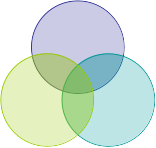
\includegraphics[]{kansei.png}
    \caption[]{Figure caption}
    \label{fig:1}
\end{figure}

All figures including photographs to be captioned below the figure, and all
tables to be captioned above the table. Captions to be justified left, aligned
with the left edge of the figure or table. Captions to be of the form;
Figure~\ref{fig:1}: Application Form for KANSEI, Table~\ref{tab:1}: Application
Form for KANSEI, etc. All figures to be numbered sequentially in accordance
with their first reference in the text. Similarly tables. Figures and tables to
be placed in the text in numbered order and as close as possible to the point
at which they are first referred to. Figures preferably to fit full width
between margins. Where this is not appropriate the figure or table should be
placed centrally on the page width. Text should not be wrapped around the
figure or table. Placing two smaller figures side by side is acceptable.
Photographs must be originals and should be pasted on the manuscript.

\subsection{Units}

SI unit systems are to be used in all text, figures and tables.

\subsection{References}

Publications, cited in the text should be collected at the end of the text. All
references should appear in order with the numbers in parentheses, such
as~\cite{ninomiya1988},~\cite{kawasima1996, kato2000} or [4-7]. Journals are to
be referred as family name(s) of author(s) preceded by the initials of first
and/or middle name, paper title and journal title (do not abbreviate the
title), number of volume (number), start- and ending page number, and published
year in parentheses. Books should be referred by the name(s) of author(s), book
title, publisher, its location, and/or referred page number, published year in
parentheses. Use the following system for arranging your references:

\begin{itemize}[noitemsep]
    \item For journals
        \begin{enumerate}[noitemsep]
            \item Y. Nagai, T. Matsumura; A Survey on Physiological Strains of Asbestos
                Abatement Work, Journal of Occupational Accidents; 2(8), pp.31-38, 1993.
        \end{enumerate}
    \item For books
        \begin{enumerate}[noitemsep]
            \setcounter{enumi}{2}
            \item R.L. Keeney, T. Suzuki and I. Kobayashi; Decisions with Multiple
                Objectives; John Wiley \& Sons, New York, pp.596-598, 1984.
        \end{enumerate}
    \item For edited books and edited proceedings of conferences, symposia,
        etc.
        \begin{enumerate}[noitemsep]
            \setcounter{enumi}{7}
            \item R.C. Willnges, M. Kubo and F. Terauchi; Design of
                Human-computer Dialogues. In; G. Salvendy (Ed.) Human-computer
                Interactions; 1st. USA-Japan Conference on Human-Computer
                Interaction, Elsevier, Amsterdam, pp.33-42 , 1984.
        \end{enumerate}
    \item For non-edited proceedings of conferences, symposia, etc.
        \begin{enumerate}[noitemsep]
            \setcounter{enumi}{14}
            \item Y. Shimizu and A. Harada; Main problem of working
                conditions and environment in small scale industry, National
                Tripartite Workshop on Improvement of Working Conditions,
                Sapporo, 1985.
        \end{enumerate}
\end{itemize}



\section*{Acknowledgments}

This work was supported by Grant-in-Aid for KANSEI Research of
Japan.

\section*{Notes}

\begin{enumerate}[noitemsep]
    \item Description of the note, if necessary.
\end{enumerate}


% This section is the references
\printbibliography[title=REFERENCES]


% Finished!
\end{document}
